% =====================================================================
%  2026-27 AIAA DBF Proposal: American University of the Middle East
%  P1, first prototype of the final proposal (31 Oct 2026). P0, the layout
%  skeleton, is archived untouched in versions/P0_base_prototype/.
%  Build:   ./build.sh            (writes the contest-named PDF here)
%  Rules:   PDF, max 6 pages, US Letter, 10 pt, 1.5 spacing, university
%           name on page 1, sections in rubric order (rules Sec. 5.1).
% =====================================================================
\def\dbfroot{../design-system}
\documentclass{dbfdoc}
% P1.2: 0.17 in more height per page for the mock-judging fixes (rules 5.1.1 set no margins);
% the page-1 band still clears: 0.70 in + 1.00 in = 1.70 in, as before.
\geometry{top=0.70in, bottom=0.58in, left=0.62in, right=0.62in, footskip=0.30in}
\makeatletter\def\dbf@mx{0.62}\def\dbf@mr{7.88}\def\dbf@tw{7.26}\makeatother
\setlength\dbffrontskip{1.00in}
\makeatletter\renewcommand\dbf@thead{\dbf@trackedsans\bfseries\fontsize{7}{8.5}\selectfont}\makeatother % table headers at 7 pt (readability note)

\dbfsetdoc{Towed-Sensor Surveillance UAV}{Proposal}{AUM-DBF-27-PRP-001}{C}
\dbfsetdate{31 Oct 2026}

% =====================================================================
%  SINGLE SOURCE OF TRUTH for the site-density numbers; every other number is generated into data/p1.tex.
%  The exec summary, glance panel, tables and text all read these macros,
%  so they can never disagree. Replace \dbftbd{...} with the value once
%  the analysis produces it (later: generated by the analysis scripts).
%  Units are SI (team decision, 11 Oct 2026): m, kg, s, m/s, Wh.
%  Rule limits are quoted with their US value in parentheses where the
%  rules define them. Scoring rounds to 2 decimals in s, in, oz, lb
%  (rules Sec. 6.2), but score ratios are unit-free. The GM drop height
%  is declared in whole inches: use 0.0254-m steps (1.524 m = 60 in).
%  Macro names keep "Weight" for continuity; the values are masses (kg).
%  Numbers the analysis computes live in data/analysis.tex instead, generated
%  by analysis/s7_export.py (12 Oct 2026). Each macro is defined in exactly one
%  of the two files: a duplicate \newcommand stops the build.
% =====================================================================

% --- Aircraft, sensor, missions and scores: GENERATED in data/p1.tex (tools/p1_data.py, P1).

% --- Fly-off site air (verified 11 Oct 2026) ----------------------------
% Site: TIMPA, 3250 N Reservation Rd, Marana AZ, 32.26474 N 111.27386 W
%   (timpa.org/location); ground elevation 667 m (2,189 ft), USGS 3DEP 1-m
%   DEM via the Elevation Point Query Service. Dates and hours: 15-18 Apr
%   2027, 07:00-18:00 local (rules Sec. 2.4, 2.5).
% Data: hourly ASOS at Tucson Intl (KTUS), 15-18 Apr 1996-2025, 2,878 obs
%   (Iowa Environmental Mesonet). Station pressure at the TIMPA elevation
%   from the altimeter setting, P = A((288 - 0.0065 h)/288)^5.2561 (NWS);
%   moist-air density from T, dew point and P.
%   At the daily high: mean 1.081, 10th percentile 1.064 kg/m^3.
%   Flying hours (07-18): mean 1.095 kg/m^3.
%   Cross-checks: Ryan Airfield (KRYN, 2008-2025) within 0.2 %; mean daily
%   high 28.0 C (82.5 F) against the NWS Tucson April normal high of
%   82.9 F (1991-2020).
% Design value = 10th percentile at the daily high: the air is thinner on
%   only 1 contest afternoon in 10. Density altitude 1,444 m (ISA).
% Supersedes Script 3's 1.051 and the airfoil study's 1.0634 (which used
%   the KTUS field elevation, 806 m, instead of TIMPA's 667 m).
\newcommand\nRho{1.064}            % kg/m^3, hot-day design density (make_charts.py reads it)
\newcommand\nRhoTypical{1.081}     % kg/m^3, mean at the daily high
\newcommand\nSiteElev{667}         % m, TIMPA ground
\newcommand\nDensityAlt{1{,}444}   % m, ISA density altitude at \nRho
% AIAA-format source footnote: put \fnRho right after the first use of \nRho in the text.
\newcommand\fnRho{\footnote{10th percentile at the daily high, 2{,}878 hourly KTUS observations, 15--18 Apr.\ 1996--2025, reduced to TIMPA (667~m). Iowa Environmental Mesonet, ``ASOS Data Download,'' retrieved 11 Oct.~2026.}}
     % site air density (the only hand-entered numbers, with method and source)
% GENERATED by proposal/tools/p1_data.py (31 Oct 2026). Do not edit: change the sources and re-run.
% Each macro: value % source key (DB-02 F-* = out/finalists/F_results.json).
\newcommand\nSpan{1.82}  % rules cap 1.829 m; DB-02 spec
\newcommand\nWingArea{1.00}  % F-A-S
\newcommand\nAR{3.31}  % F-A-AR
\newcommand\nMAC{0.555}  % F-A-MAC
\newcommand\nRootChord{0.646}  % F-A-CR
\newcommand\nTipChord{0.452}  % F-A-CT
\newcommand\nLength{1.60}  % F-A-LEN
\newcommand\nEmptyMass{6.96}  % F-A-EMPTY (DB-01 fit, estimate)
\newcommand\nGrossMtwo{14.6}  % 120-draw median g2
\newcommand\nGrossMthree{10.5}  % 120-draw median g3
\newcommand\nStallMtwo{11.9}  % F-A-VS2
\newcommand\nStallMthree{10.1}  % 120-draw median vs3
\newcommand\nCLmaxLand{1.93}  % F-A-CLMAX (NACA TR 534 + TN 663 method, estimate)
\newcommand\nStaticMargin{16}  % F-A-SMMIN/SMMAX 16.0-16.1 % MAC
\newcommand\nXcg{0.433}  % F-A-XCG
\newcommand\nXnp{0.521}  % F-A-XNP
\newcommand\nSh{0.291}  % F-A-SH
\newcommand\nSv{0.069}  % F-A-SV
\newcommand\nTailArm{1.05}  % F-A-LT
\newcommand\nPackWh{97.7}  % TP3300-8SE55 datasheet, 8S 3300 mAh (DB-02 A-03)
\newcommand\nUsableWh{78.1}  % 80 % usable, sizing.toml
\newcommand\nThrust{101}  % F-PROP-T0
\newcommand\nTWstatic{0.71}  % 120-draw median tw2
\newcommand\nDeclMed{6.25}  % median declaration, finalists_rows S10F8
\newcommand\nDeclLo{4.5}  % P10
\newcommand\nDeclHi{7.5}  % P90
\newcommand\nContainer{1.18}  % S8 container for 8 kg
\newcommand\nMtwoPayload{7.4}  % median M2 payload
\newcommand\nMtwoTimeDP{204}  % design point five-lap time (p1_nominal m2.t5)
\newcommand\nMtwoTime{231}  % median t2
\newcommand\nMtwoTimeLo{158}  % P10
\newcommand\nMtwoTimeHi{287}  % P90
\newcommand\nMtwoV{29}  % design point
\newcommand\nMtwoBank{71}  % design point
\newcommand\nMtwoN{3.07}  % design point
\newcommand\nMtwoLap{38.9}  % design point
\newcommand\nMtwoWh{77.9}  % design point energy
\newcommand\nMthreeLaps{6}  % median laps
\newcommand\nMthreeLapsLo{5}  % P10
\newcommand\nMthreeLapsHi{9}  % P90
\newcommand\nMthreeMass{3.4}  % median flown M3 sensor
\newcommand\nMthreeProd{20.7}  % median laps x mass
\newcommand\nMthreeProdLo{16.6}  % P10
\newcommand\nMthreeProdHi{25.8}  % P90
\newcommand\nMthreeV{25}  % design point at the median mass
\newcommand\nMthreeN{3.24}
\newcommand\nMthreeLap{39.9}
\newcommand\nStowMed{16.5}  % stow at the median M3 mass
\newcommand\nStowEight{24.6}  % stow at 8 kg
\newcommand\nDrop{1.524}  % rules cap 60 in
\newcommand\nDropIn{60}
\newcommand\nGMprod{9.53}  % median declaration x 1.524 m
\newcommand\nTow{2.73}  % 1.5 x span
\newcommand\nTowDesign{2.83}  % rule minimum + dr_trade deploy margin
\newcommand\sMtwo{1.46}  % F-A-M2
\newcommand\sMthree{2.85}  % F-A-M3
\newcommand\sGM{1.44}  % F-A-GM
\newcommand\sTotal{6.76}  % F-A-MEAN
\newcommand\sTotalPten{6.25}  % F-A-P10
\newcommand\sPtop{0.313}  % F-A-PTOP
\newcommand\sPfirst{0.369}  % F-A-P1ST (report 90)
\newcommand\sPtopB{0.295}  % F-B-PTOP
\newcommand\sTotalB{6.71}  % F-B-MEAN
\newcommand\sPtopPct{31}  % F-A-PTOP in %
\newcommand\sPtopCtlPct{13}  % F-C-PTOP in %
\newcommand\nMGTOW{16.1}  % heaviest loading: M2 at declared max (variants_geometry.json)
\newcommand\sPtopCtl{0.128}  % F-C-PTOP
\newcommand\sTotalCtl{6.33}  % F-C-MEAN
\newcommand\sPtopAlow{0.251}  % F-A-PTOP-fowler_low
\newcommand\sBreakeven{0.29}  % F-AB-BREAKEVEN
\newcommand\sRegA{0.044}  % F-A-MAXREG
\newcommand\sRegB{0.018}  % F-B-MAXREG
\newcommand\sFieldMed{6.62}  % F-FLD-2027-P50
\newcommand\sFieldLo{6.22}
\newcommand\sFieldHi{7.04}
\newcommand\sFieldGM{11.4}  % F-FLD-GMRIV
\newcommand\sWinLo{5.61}  % F-BT-*-WIN
\newcommand\sWinHi{6.80}  % F-BT-*-WIN
\newcommand\tRef{6.76}  % p1_sens tornado ref (= F-A-MEAN)
\newcommand\tLapUp{0.54}  % lap factor +10 %, loss
\newcommand\tLapDn{0.27}  % lap factor -10 %, gain
\newcommand\tRhoDn{0.22}  % density -10 %, loss
\newcommand\tEtaDn{0.22}  % efficiency -10 %, loss
\newcommand\tMassUp{0.16}  % airframe +10 %, loss
\newcommand\tMassUpTwenty{0.39}  % airframe +20 %, loss
\newcommand\tAreaMax{0.02}  % wing area +-10 %
\newcommand\tClDn{0.08}  % CLmax -10 %, loss
\newcommand\tFieldUp{0.07}  % field +10 %, loss
\newcommand\tFrozenBest{6.33}  % frozen sweep max
\newcommand\tFrozenM{4}
\newcommand\tDeclGain{0.42}  % tech declaration gain
\newcommand\tFeasEight{0.55}  % frozen 8 kg P(M2 feasible)
\newcommand\tCompletion{55}  % s6 trade weights
\newcommand\bAirframe{1{,}760}  % Prototype airframe, test rigs and tools (PR-01) [PR-01]
\newcommand\bComp{1{,}320}  % Competition airframe and Variant B wing kit [est.]
\newcommand\bFowler{180}  % Fowler tracks, carriages, test section [est.]
\newcommand\bPropulsion{2{,}850}  % Motors, ESCs, radio, servos (PR-01) [PR-01]
\newcommand\bBatteries{1{,}950}  % 8S packs, chargers, sacks, 58 V fuses [PR-01]
\newcommand\bSensor{550}  % Sensor lights, drum, slip ring, test box [PR-01]
\newcommand\bTungsten{520}  % Tungsten alloy ballast, 8 kg [online average]
\newcommand\bContainers{240}  % Containers, simulators, drop rig [PR-01]
\newcommand\bConsumables{460}  % Spare props, adhesives, consumables [PR-01]
\newcommand\bCrating{150}  % Shipping crate [PR-01]
\newcommand\bHazmat{100}  % Paint, glue, solvent bought in Tucson [est.]
\newcommand\bAirfare{10{,}820}  % Airfare, Kuwait--Tucson, 7 travellers [quote]
\newcommand\bLodging{2{,}850}  % Lodging, 6 nights, 4 rooms [quote]
\newcommand\bMeals{3{,}640}  % Meals, 7 travellers, GSA Tucson rate [GSA]
\newcommand\bGround{1{,}200}  % Van hire, fuel, excess baggage for the crate [est.]
\newcommand\bVisas{3{,}050}  % US visa fees, 7 travellers [fee]
\newcommand\bFees{1{,}420}  % Fly-off fee, AIAA student dues, pilot AMA dues [rules, fee]
\newcommand\bHwproto{1{,}760}  % hwProto [group]
\newcommand\bHwcomp{1{,}500}  % hwComp [group]
\newcommand\bHwmotors{2{,}850}  % hwMotors [group]
\newcommand\bHwpacks{1{,}950}  % hwPacks [group]
\newcommand\bHwairframe{3{,}260}  % hwAirframe [group]
\newcommand\bHwpower{4{,}800}  % hwPower [group]
\newcommand\bHwpayload{1{,}320}  % hwPayload [group]
\newcommand\bHwcrate{250}  % hwCrate [group]
\newcommand\bSubtotal{33{,}070}  % sum of printed rows
\newcommand\bContingency{4{,}960}  % 15 %
\newcommand\bTotal{38{,}030}  % sum of printed rows
\newcommand\bTotalK{38.0}  % total, thousands
\newcommand\bTravellers{7}  % team lead, 31 Oct
\newcommand\bAirfareEach{1{,}545}  % quote, whole dollars
\newcommand\bRooms{4}  % 2 per room
\newcommand\bMembers{21}  % team lead, 31 Oct
\newcommand\bTungstenKg{66}  % mean of 6 heavy-alloy listings
\newcommand\bTungstenN{6}
\newcommand\bVisa{435}  % MRV 185 + integrity fee 250
\newcommand\bMIE{80}  % GSA FY2027 Tucson M&IE
\newcommand\bFundKWD{10{,}000}  % team lead, 31 Oct
\newcommand\bFundUSD{32{,}170}  % at 0.310829 KWD/USD
\newcommand\bBalance{5{,}860}  % total minus the 10,000 KWD allocation
\newcommand\nCma{$-$0.61}  % AVL about the CG (p1_data.avl_cg)
\newcommand\nCnb{0.076}  % AVL about the CG
\newcommand\nClb{$-$0.012}  % AVL about the CG
\newcommand\nCLa{3.80}  % AVL
\newcommand\nCDzero{0.0216}  % p1_nominal m2.cd0 (wing + body)
\newcommand\nLDcruise{9.8}  % M2 level flight at the design-point speed
\newcommand\nLDmax{10.5}  % 1 / (2 sqrt(CD0 k))
\newcommand\nPowerMtwo{1.4}  % M2 mean battery power, kW (design point)
\newcommand\nAmpsMtwo{47}  % M2 mean current at 8S nominal 29.6 V
\newcommand\nMtwoGrossDP{14.4}  % design-point M2 gross
\newcommand\nMthreeGrossDP{10.3}  % design-point M3 gross at the median flown mass
\newcommand\nTensionMed{107}  % m g n at the median M3 mass, design-point n
\newcommand\nTensionEight{254}  % m g n at 8 kg, same n
\newcommand\sExpected{4.83}  % A total with failed attempts sampled (field_stats)
\newcommand\sExpectedCtl{4.01}  % first iteration, same
\newcommand\tSpanEDn{0.13}  % span efficiency -10 %, loss
\newcommand\sPMtwoDone{0.82}  % F-A-PM2D
\newcommand\sPMthreeDone{0.54}  % F-A-PM3D
\newcommand\sFieldGMexp{9.14}  % expected-field GM best, kg m (s6.fields)
\newcommand\sFieldMthreeExp{20.2}  % expected-field M3 best, lap kg (s6.fields)
\newcommand\sTrailLo{0.012}  % finalists vs A, paired
\newcommand\sTrailHi{0.033}
\newcommand\sPtopFtwelve{0.300}  % 1.2 m2 Fowler
\newcommand\pSimFeas{0.06}  % P(M2 feasible), one simulator at a 6 kg declaration
\newcommand\pMthreeLo{3.25}  % M3 per-attempt optimum, within 0.01
\newcommand\pMthreeHi{4.25}
\newcommand\pStowFree{0.009}  % mean-total gain if the stow fell outside the window
          % every other number: generated by tools/p1_data.py from DB-02 and analysis results
% GENERATED by tools/p1_ga.py: team GA drawings present or not.
\newcommand\gaStatus{}
\newcommand\gaThumb{}
          % team GA drawing status and glance thumbnail: generated by tools/p1_ga.py

\usepackage{needspace}
\begin{document}

\begin{frontmatter}
% =====================================================================
%  1.0 EXECUTIVE SUMMARY  (5 pts)   P1.2, 31 Oct 2026
%  Rubric (5.1.4):  [x] Objective statement
%                   [x] Planned approach to achieve all objectives
%                   [x] Main points from every subsequent section (budget and funding included, P1.2)
% =====================================================================
\section{Executive Summary}
% P1.2: the side panel became a full-width readout strip so page 1 no longer grows with the panel
% (and stays fixed when the team's drawings arrive; the GA plate in 3.4 carries them).
\newcommand\gl[3]{\parbox[t]{0.163\linewidth}{\raggedright
  {\dbflabelfont\fontsize{7}{8.4}\selectfont\color{dbfFog}\MakeUppercase{#1}}\par\vspace{2pt}%
  {\dbftablefont\bfseries\fontsize{12.5}{14.5}\selectfont\color{white}#2}\hspace{0.2em}{\sffamily\fontsize{7.6}{9}\selectfont\color{dbfFog}#3}}}
\textbf{Objective.} Machine Masters will design, build and fly a hand-flown electric aircraft that delivers the sensor in its container (Mission~2), tows it through its light sequence and recovers it (Mission~3), and protects it in the Ground Mission drop, to post the highest total score at Tucson in April 2027.

\textbf{Approach.} The rules became 21 subsystem requirements. A mission model calibrated on the 2022--26 fly-offs flew 162 candidate aircraft through every mission, failed attempts included, against simulated rival fields; completion pays 4.5 of 7.5 points, so reliability carries \tCompletion\,\% of the trade weight. Sensor and container are built for 3--8~kg, with the maximum declared at inspection ($+$\tDeclGain{} points over fixing it at design).

\textbf{Design.} A \nSpan~m, \nWingArea~m² high wing with Fowler flaps ($C_{L,\max}$ \nCLmaxLand), conventional tail, fixed tricycle gear and one 8S tractor stalls at \nStallMtwo~m/s at its \nGrossMtwo~kg Mission~2 mass. It waives Mission~1, carries one \nMtwoPayload~kg sensor container, tows \nMthreeMass~kg and drops the declared sensor from \nDrop~m: \sTotal{} of 7.5 with every mission completed and the field's highest mission total in \sPtopPct\,\% of simulated contests, failed attempts counted (first iteration \sPtopCtlPct\,\%); a slotted 1.2~m² wing is the fallback.

\textbf{Execution.} Six sub-teams build two airframes of laser-cut ply and balsa on carbon tubes, retire the top risks in 14 bench and flight tests by 15~January, fly the prototype at least 20 times and freeze the design on 19~February; the \$\bTotalK{}k budget, travel included, is fully funded by the university.

\vspace{6pt}\noindent\begin{dbfinkpanel}[Design at a glance / Variant A]
\gl{Wingspan}{\nSpan}{m}\hfill\gl{Wing area}{\nWingArea}{m²}\hfill\gl{M2 gross mass}{\nGrossMtwo}{kg}\hfill\gl{Stall, M2}{\nStallMtwo}{m/s}\hfill\gl{Score, if done}{\sTotal}{/ 7.5}\hfill\gl{P(top of field)}{\sPtop}{}
\end{dbfinkpanel}

\end{frontmatter}

% =====================================================================
%  2.0 MANAGEMENT SUMMARY  (20 pts)           budget: ~1.15 pages, ~250 words
%  Rubric (5.1.4):  [ ] Organization, roles of each team, individual skill sets
%                   [ ] Organization chart (by team/function; no names needed)
%                   [ ] Schedule / major milestone chart
%                   [ ] Budget: materials AND travel AND all other expenses
%  Judges 2026: itemize test articles, crating, spare props, adhesives and
%  consumables; tie funding to a CONFIRMED amount; include contingency.
%  Layout: the two full-width floats (roles table, Gantt) are defined here,
%  at the top of the section, so they land at the top of page 2.
% =====================================================================
\section{Management Summary}

\begin{table*}[t]
\caption{Sub-team responsibilities and the skill sets each requires.}\label{tab:roles}
\begin{dbftable}{colspec={Q[l,wd=1.45in] X[1.3,l] X[1,l]}}
Sub-team & Responsibility & Required skills \\
Aero \& Performance & Sizing, lap and energy model, stability and control & \dbftbd{skills} \\
Structures \& Manufacturing & Airframe design, layup and build, load tests & \dbftbd{skills} \\
Propulsion \& Avionics & Motor, propeller, battery, ESC, radio and fail-safe & \dbftbd{skills} \\
Sensor Systems & Sensor, D\&R reel, shipping container, rigging & \dbftbd{skills} \\
Flight Operations & Pilot, observer, ground crew, checklists & \dbftbd{skills} \\
Business \& Logistics & Budget, sponsorship, travel, documentation & \dbftbd{skills} \\
\end{dbftable}
\end{table*}

\begin{figure*}[t]
\dbfplaceholder{\textwidth}{1.5in}{Gantt / full width / lanes: design, manufacturing, test, reports, competition}
\caption{\dbftbd{takeaway}. Milestones: proposal 31 Oct; Q\&A rounds from 1 Nov; PDR; CDR; prototype first flight; sensor bench test; design report 19 Feb; competition aircraft first flight; Pre-Tech/First-Flight certification; fly-off 15--18 Apr.}\label{fig:gantt}
\end{figure*}

\subsection{Team Organization}
\dbfnote{About 110 words. Functional structure: Team Lead and Chief Engineer, with the Faculty Advisor above; why Sensor Systems exists this year; how decisions are made (weekly leads meeting, PDR/CDR gates); requirement-ID traceability. Refer to Fig.~\ref{fig:org} and Table~\ref{tab:roles}.}
\dbffill{110}

\begin{figure}[t]
\dbfplaceholder{\columnwidth}{1.35in}{Org chart / by function / no names}
\caption{\dbftbd{takeaway}: one owner for every scored subsystem.}\label{fig:org}
\end{figure}

% Budget/funding float sources sit here, ahead of the 2.2/2.3 text, so that
% they land inside Section 2.0 (verified by the sequence guard in build.sh).
\begin{table}[t]
\caption{Program budget, all costs including travel (USD).}\label{tab:budget}
\begin{dbftable}{colspec={X[l] Q[r] Q[r]}, row{Z}={font=\dbftotalrow}, hline{Y}={0.4pt,dbfGraphite}}
Category & Cost & Share \\
Airframe materials and prototypes & \dbftbd{\$} & \dbftbd{\%} \\
Propulsion, avionics, radio & \dbftbd{\$} & \dbftbd{\%} \\
Batteries, charging sacks, fuses & \dbftbd{\$} & \dbftbd{\%} \\
Sensor electronics and lights & \dbftbd{\$} & \dbftbd{\%} \\
Containers, simulators, drop rig & \dbftbd{\$} & \dbftbd{\%} \\
Spares, props, adhesives, consumables & \dbftbd{\$} & \dbftbd{\%} \\
Crating and shipping & \dbftbd{\$} & \dbftbd{\%} \\
Travel: flights, lodging, transport & \dbftbd{\$} & \dbftbd{\%} \\
Fly-off fee, AIAA/AMA memberships & \dbftbd{\$} & \dbftbd{\%} \\
Contingency (\dbftbd{\%}) & \dbftbd{\$} & \dbftbd{\%} \\
Total & \dbftbd{\$} & 100\% \\
\end{dbftable}
\end{table}

\begin{table}[t]
\caption{Funding sources and status.}\label{tab:funding}
\begin{dbftable}{colspec={X[l] Q[r] Q[l]}, row{Z}={font=\dbftotalrow}, hline{Y}={0.4pt,dbfGraphite}}
Source & Amount & Status \\
\dbftbd{college allocation} & \dbftbd{\$} & \dbftbd{confirmed?} \\
\dbftbd{sponsor} & \dbftbd{\$} & \dbftbd{pending?} \\
Total & \dbftbd{\$} & \\
\end{dbftable}
\end{table}

\subsection{Schedule and Milestones}
\dbfnote{About 60 words. Built backward from the fly-off; prototypes; internal PDR/CDR gates; owners and pass criteria per milestone. Refer to Fig.~\ref{fig:gantt}.}
\dbffill{60}

\subsection{Budget}
\dbfnote{About 80 words. Every expense, including Kuwait--Tucson travel; the funding sources and which are confirmed; the contingency rationale. Refer to Table~\ref{tab:budget} and Table~\ref{tab:funding}.}
\dbffill{80}

% =====================================================================
%  3.0 CONCEPTUAL DESIGN APPROACH  (55 pts)   P1.2, 31 Oct 2026
%  Rubric (5.1.4):  [x] Decomposition of mission reqs into subsystem reqs (3.1, Table 03)
%                   [x] Trade studies conducted, with results (3.3, Tables 04-05, Figs. 05-06)
%                   [x] Preliminary design / sizing results; concept sketch (3.4, Figs. 07-08, Table 06)
%                   [x] Sensitivity study of design parameters (3.2, Figs. 03-04)
%                   [x] Design approach per mission WITH initial targets (3.5, Table 07)
%  Numbers: data/p1.tex. Figures: tools/p1_figures.py. Table 03 clause sources: rules of 2 Sep 2026
%  (Secs. 3.1-3.3, 4.2). Table 04 evidence: DB-01 trades (analysis/out/trades_report.txt: audited matrices
%  with sensitivity weights; config_trades_report.txt) and DB-02 rev B (finalists, 30 Oct; S-06 airfoil;
%  A-04 tail and fail-safe). P1.2 applies the mock-judging notes of 31 Oct
%  (claude_docs/proposal_mock_judging_2026-10-31.md): one basis per table, alternatives shown,
%  Cm_alpha about the CG, the payload trades charted, the stow read as outside the window.
% =====================================================================
\needspace{4\baselineskip}
\section{Conceptual Design Approach}

% ---------------------------------------------------------------------
\subsection{Mission Requirements Decomposition}
Each mission score and rule became a numbered subsystem requirement (SR, Table~\ref{tab:decomp}); the SR column of Table~\ref{tab:tests} shows the test that verifies each.

\begin{table*}[t]
\caption{Mission requirements decomposed into subsystem requirements (SR). \textsuperscript{†}\,Team requirement beyond the rules.}\label{tab:decomp}
\begin{dbftable}{colspec={Q[l,wd=0.52in] Q[l,wd=1.08in] X[0.95,l] X[1.8,l]}}
Mission & Score & Key constraints & Derived subsystem requirements \\
M1 Staging & $M_1 = 1.0$ & 3 laps in 5 min; may be waived and credited by a successful M2 & SR-01 static margin \nStaticMargin\,\% MAC in every loading\textsuperscript{†}; SR-02 all checks inside the 5-min staging \\
M2 Delivery & $M_2 = 1 + \frac{W/t}{(W/t)_{\max}}$ & Container plus simulators at the declared maximum; TOP up; 5 laps & SR-03 bay for a 288\,$\times$\,303\,$\times$\,303~mm container; SR-04 positive restraint; SR-05 CG inside marked limits in every loading \\
M3 Sensor & $M_3 = 2 + \frac{N W_s}{(N W_s)_{\max}}$ & Internal until deployed, before the first downwind turn; OFF, SOLID, FLASHING, OFF; stow to land & SR-06 internal drum, tow $\geq$ \nTow~m, latched stow; SR-07 three lights, modes over the line, visible in sun; SR-08 no divergent swing at $n$ = \nMthreeN; SR-09 own COTS battery; SR-10 line clear of propeller, tail\textsuperscript{†}; SR-11 same door state every mission \\
Ground & $GM = 0.5 + \frac{W_s h}{(W_s h)_{\max}}$ & 6 drops on concrete, $h \leq$ 1.524~m (60~in); ring to bottom $<$ 381~mm (15~in); 5-min rigging & SR-12 container absorbs $W_s h$, sensor designed for 150~g; SR-13 tool-less O/E rigging, flush fittings; SR-14 test box drives all three modes \\
System & -- & Span $\leq$ 1.829~m (6~ft); TOGW $<$ 24.95~kg (55~lb); $\leq$ 100~Wh; no autopilot, GPS or camera; arming, fuse, radio rules & SR-15 pilot-in-the-loop only; SR-16 positive latches, no magnets; SR-17 §4.2.5 fail-safe, range check; SR-18 structure for $n$ = \nMthreeN{} and tip lift; SR-19 top arming plug $\geq$ 152~mm aft of the propeller plane, external Rx switch, separate Rx pack, BEC off, fuse $\leq$ pack rating; SR-20 M2 at full payload within \nUsableWh~Wh usable, stall $\leq$ 12~m/s; SR-21 ESC, pack within rated temperature\textsuperscript{†} \\
\end{dbftable}
\end{table*}

% ---------------------------------------------------------------------
\subsection{Scoring Model and Sensitivity Study}
The mission score sums four terms, each a completion credit plus a ratio to the best result in the field, our own included:\footnote{AIAA, \emph{2026--27 Design, Build, Fly Rules}, 2 Sep.~2026, Secs.~3.1--3.3, 6.3.}
\begin{equation}
\begin{aligned}
S_\mathrm{M} &= M_1 + \Bigl[1 + \tfrac{(W/t)}{(W/t)_\mathrm{max}}\Bigr]
  + \Bigl[2 + \tfrac{N W_s}{(N W_s)_\mathrm{max}}\Bigr] \\
 &\quad + \Bigl[0.5 + \tfrac{W_s h}{(W_s h)_\mathrm{max}}\Bigr] \leq 7.5
\end{aligned}
\end{equation}
Completion is worth 4.5 points and the bonuses at most 3.0, yet in 2026 only 17 of 83 inspected teams completed every mission;\footnote{AIAA, ``DBF Competition Summaries,'' 2022--2026 (513 team results).} winning totals ran \sWinLo--\sWinHi{} in 2022--26. The declared sensor mass $W_s$ sets the Ground Mission product, every Mission~2 container and the Mission~3 ballast cap.

Each design flies 120 random draws of every uncertain input (mass, $C_{L,\max}$, drag, efficiency, density and a lap-time factor from 24 measured flights\footnote{Predicted and measured times in seven DBF design reports, 2021--26; airframe masses of 14 top-three aircraft, 2022--26.}) against 5{,}000 simulated rival fields with attempt success from 2023--26; these inputs describe pilots and staging, not the payload, so they carry over and are refitted to the prototype's laps (TC-10). Efficiency, airframe mass and span efficiency lead the design parameters (Fig.~\ref{fig:sens}; \tEtaDn, \tMassUp{} and \tSpanEDn{} points per 10\,\%), and 10\,\% slower laps cost \tLapUp. Mission~2 uses \nMtwoWh{} of the \nUsableWh~Wh usable, leaving the 20\,\% reserve untouched. Declaring at inspection is the largest lever (Fig.~\ref{fig:declared}): fixed at design the best is \tFrozenBest{} (\tFrozenM~kg); declared, \sTotal{} with every mission completed.

\begin{figure}[t]
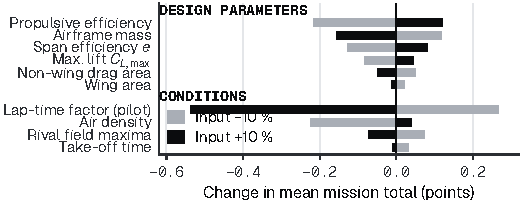
\includegraphics{figures/fig_tornado.pdf}
\caption{Mean mission total change for $\pm$10\,\% on each input: lap time and density, which the team does not set, outweigh every design parameter.}\label{fig:sens}
\end{figure}

\begin{figure}[t]
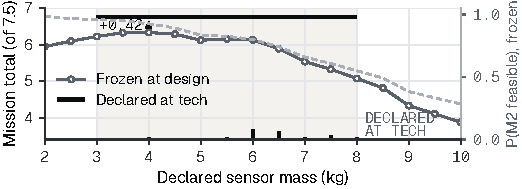
\includegraphics{figures/fig_declared.pdf}
\caption{Declaring at inspection is worth $+$\tDeclGain{} over the best mass fixed at design; fixed at 8~kg, Mission~2 is feasible on only \tFeasEight{} of airframes. Shaded: 3--8~kg window; bars: masses the draws declare.}\label{fig:declared}
\end{figure}

% ---------------------------------------------------------------------
\subsection{Configuration Trade Studies}
Trade weights come from the sensitivity study (completion \tCompletion\,\%, lap performance 17\,\%, high lift 10\,\%, airframe mass 7\,\%, efficiency 5\,\%, induced drag 4\,\%, structure and parasite drag 1\,\% each). The eleven best of 162 combinations of area, flap, declared range and propulsion were re-flown on all 120 draws (Fig.~\ref{fig:screen}) and had to hold Mission~3 completion within 10\,\% of the best and a worst-10\,\% total above the first iteration's. The 1.0~m² Fowler wing leads every finalist by \sTrailLo--\sTrailHi{} in P(top), the chance of the field's highest mission total, each paired 95\,\% interval above zero.\footnote{Flaps: R.~C. Platt, NACA Rept.~534, 1935; C.~J. Wenzinger and T.~A. Harris, NACA Rept.~664, 1939; method validated on NACA TN~663. Airfoils: M.~S. Selig et al., UIUC Low-Speed Airfoil Tests.} Table~\ref{tab:config} gives the other decisions: SD7037 is within 6\,\% of the best cruise $L/D$ of 13 sections (XFoil, $Re$ $5\times10^{5}$) and keeps its maximum lift tripped (UIUC), while the turn-lift leaders lose 15--52\,\% at $C_L$ 0.4. Fig.~\ref{fig:payload} and Table~\ref{tab:dr} give the payload and drum trades.

\begin{table}[t]
\caption{Configuration decisions. Points: change in mean mission total; matrix: weighted score of 100, team criteria weighted by the sensitivity study (top weights shown).}\label{tab:config}
\begin{dbftable}{colspec={Q[l,wd=0.50in] Q[l,wd=0.66in] X[l]}, colsep=3pt, cell{2-Z}{2}={font=\dbftotalrow}}
Decision & Selected & Alternatives, evidence \\
Planform & Straight & Delta $-$1.69, biplane $-$0.32 \\
Flap & Fowler, 1.0 & P(top) \sTrailLo--\sTrailHi{} lower \\
Airfoil & SD7037 & $L/D$ 73/92/96 at $C_L$ 0.4/0.6/1.0; trip-proof \\
 & & Of 13: E387 62/85/118, MH 114 35/64/119 \\
Wing & High, 90 & Low 71, mid 53 (bay 30\,\%, clearance 24\,\%) \\
Tail & Conv., 83 & T 73, twin boom 68 (line clearance 36\,\%); V: §4.2.5 fail-safe relies on mixing \\
Gear & Trike, 85 & Taildragger 76, bicycle 51 (landing 43\,\%) \\
Power & One 8S & 12S $-$0.02, twin $-$0.05 in P(top) \\
Tips & Plain & Winglets $-$0.01 to $-$0.05 \\
Sensor & At tech & Frozen $-$\tDeclGain{} (Fig.~\ref{fig:declared}) \\
\end{dbftable}
\end{table}


\begin{figure}[t]
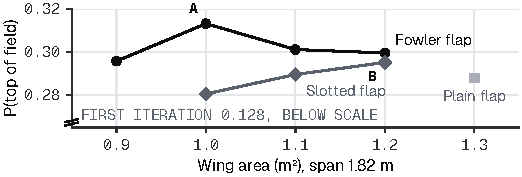
\includegraphics{figures/fig_screen.pdf}
\caption{Finalists on the same 120 draws: the 1.0~m² Fowler wing (A) leads; the slotted 1.2~m² wing (B) is the fallback. The axis starts at 0.265; each gap has its paired 95\,\% interval above zero.}\label{fig:screen}
\end{figure}

\begin{figure}[t]
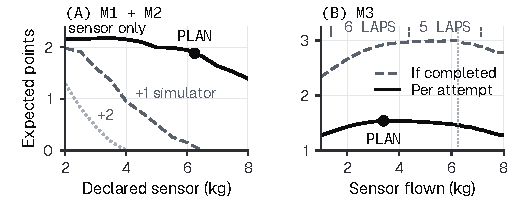
\includegraphics{figures/fig_payload.pdf}
\caption{Payload trades: (a) Mission 1 and 2 points against declared mass, 0 to 2 simulators; (b) Mission~3 points against sensor mass flown; dotted: 6.25~kg declared.}\label{fig:payload}
\end{figure}

\begin{table}[t]
\caption{Deployment-and-recovery trade (scores 1--5). Weights are the mission points at stake; the closed drum wins 99.5--100\,\% of 5{,}000 draws with estimates and weights randomised. Boom, wireless, bridle, pulley and spring reel failed the rules or the 20~s limit.}\label{tab:dr}
\begin{dbftable}{colspec={X[l] Q[c] Q[c,wd=0.42in] Q[c,wd=0.42in] Q[c,wd=0.42in]}, column{3}={bg=dbfAccentTint}, cell{1}{3}={bg=dbfInk, fg=white}, row{Z}={font=\dbftotalrow}, hline{Y}={0.4pt,dbfGraphite}}
Criterion & Wt. & Closed drum & Open drum & Free spool \\
Recovery reliability & 0.75 & 5.0 & 4.4 & 3.6 \\
Manufacturability & 0.15 & 3.1 & 5.0 & 1.7 \\
Weight, volume & 0.04 & 5.0 & 4.9 & 2.4 \\
Signal path & 0.03 & 5.0 & 5.0 & 5.0 \\
Deploy, stow time & 0.03 & 4.5 & 5.0 & 5.0 \\
Weighted total & 1.00 & \dbfselected{4.70} & 4.55 & 3.35 \\
\end{dbftable}
\end{table}

% ---------------------------------------------------------------------
\subsection{Preliminary Design and Sizing}
\subsubsection{Sizing method}
Sizing uses the hot-day density\fnRho{} of \nRho~kg/m³ and a lap model of the 152.4~m (500~ft) legs, 180° turns and downwind 360°, with stall $\leq$ 14~m/s, load factor $\leq$ 4, battery power, the 100~Wh cap and the measured $\times$1.15 lap factor. Mission~2 sits on its \nMtwoV~m/s, $n$ = \nMtwoN{} turn line at full thrust (Fig.~\ref{fig:constraint}); Mission~3 is energy-limited. Of 1{,}575 motor, propeller and pack combinations, 74 meet the turn limits and 40 were flown through the mission model; the AT7215 with a 20$\times$15E on 8S ranks first, 0.02--0.03 points ahead of a 21$\times$13E or a 12S pack, with \nThrust~N static thrust and \nPowerMtwo~kW (\nAmpsMtwo~A) mean power in Mission~2.\footnote{T-Motor and APC published test data; the model is within 3.5\,\% of a measured 2023 Mission~2 power.}

\begin{figure}[t]
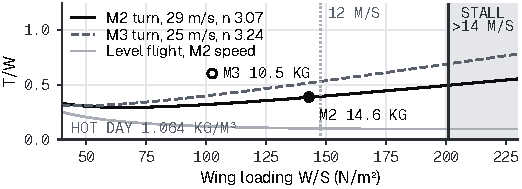
\includegraphics{figures/fig_constraint.pdf}
\caption{Mission~2 is sized by the race turn at full thrust; the Fowler flap keeps its \nGrossMtwo~kg landing under 12~m/s.}\label{fig:constraint}
\end{figure}

\begin{figure}[t]
\begin{dbfplate}{General arrangement / Variant A}{Span 1.82 m}
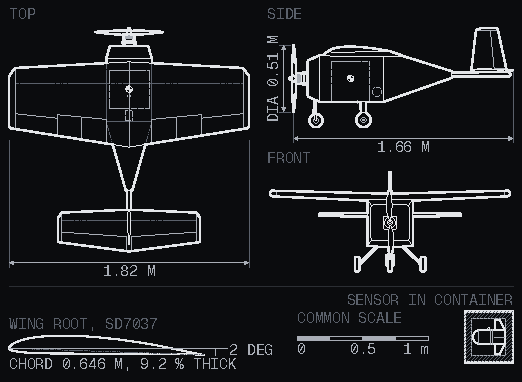
\includegraphics[width=\linewidth]{figures/fig_threeview.pdf}
\end{dbfplate}
\caption{Variant A to scale (AVL geometry; length from the propeller plane). Dashed: 8~kg container, drum, tow exit; quartered circle: CG. Below: wing root; sensor in its container.\gaStatus}\label{fig:concept}
\end{figure}

\subsubsection{Aircraft concept}
Variant A puts a straight wing (Fig.~\ref{fig:concept}, Table~\ref{tab:params}) on a 0.345\,$\times$\,0.355~m box fuselage with a conventional tail on a \nTailArm~m arm. The span sits 9~mm inside the 1.829~m limit (tip caps trimmed at weigh-in) and the area is the 1.00~m² of Fig.~\ref{fig:screen}, so the aspect ratio is \nAR. With the bay centred on the CG and the tow exit 50~mm aft, every loading flies at \nStaticMargin\,\% static margin; about the CG, AVL gives $C_{m\alpha}$ \nCma, $C_{n\beta}$ \nCnb{} and $C_{l\beta}$ \nClb{} per rad.\footnote{M.~Drela and H.~Youngren, AVL 3.52; M.~Drela, XFoil 6.99; MIT.} Variant B changes only the wing (1.2~m², slotted), tail and boom.

\begin{table}[t]
\caption{Design parameters, Variant A. Gross masses and stall speeds are medians of 120 draws, so they do not add up.}\label{tab:params}
\begin{dbftable}{colspec={X[l] Q[r] Q[l]}}
Parameter & Value & Unit \\
Span / area / aspect ratio & \nSpan{} / \nWingArea{} / \nAR & m, m² \\
Mean chord / tail arm & \nMAC{} / \nTailArm & m \\
Tail areas, H / V & \nSh{} / \nSv & m² \\
Empty mass with pack (fit) & \nEmptyMass & kg \\
Gross mass, M2 / M3 & \nGrossMtwo{} / \nGrossMthree & kg \\
Trimmed landing $C_{L,\max}$ & \nCLmaxLand & -- \\
Stall, M2 / M3 & \nStallMtwo{} / \nStallMthree & m/s \\
$C_{D0}$ / $L/D$, M2 level & \nCDzero{} / \nLDcruise & -- \\
Static margin / $C_{m\alpha}$ & \nStaticMargin{} / \nCma & \%, /rad \\
Static thrust / 8S pack & \nThrust{} / \nPackWh & N, Wh \\
M2 mean power / current & \nPowerMtwo{} / \nAmpsMtwo & kW, A \\
Tow line, built / minimum & \nTowDesign{} / \nTow & m \\
\end{dbftable}
\end{table}

\subsubsection{Sensor and D\&R system}
The sensor is a finned dart with a tungsten core (190~mm long, 85~mm body, 205~mm fins at 8~kg), towed from an eye above its CG so it flies level;\footnote{J.~Barrowman, ``Theoretical Prediction of the Center of Pressure,'' NARAM-8, 1966.} its potted electronics are designed for 150~g, checked by accelerometer in the drop tests, and a 1S pack drives three LED arrays of about 220~cd. A closed-loop servo drum (Table~\ref{tab:dr}) with a slip ring deploys 3.4~kg in about 10~s and stows it in \nStowMed~s (\nStowEight~s at 8~kg) into a latched dock. In a \nMthreeN~g turn the line carries \nTensionMed~N at 3.4~kg and \nTensionEight~N at 8~kg and is rated for four times the 3~g load. Towed 50~mm aft of the CG, the sensor keeps every loading at 16.0--16.1\,\% static margin; its 1.7~N trailing pull 0.18~m below the CG shifts $C_m$ by under 0.002 (estimate).

\subsubsection{Container and rigging}
Built once for the top of the range, the 288\,$\times$\,303\,$\times$\,303~mm container wraps the 205~mm fin span in 41~mm of polyethylene foam per face, keeping the sensor under 150~g in a 1.524~m drop with the ring under 381~mm from every face;\footnote{U.S. Dept.\ of Defense, \emph{MIL-HDBK-304B, Package Cushioning Design}, 1978.} pads are re-cut at inspection and simulators trim to 28~g.

% Targets table placed before 3.5 text so it lands before the 4.0 heading.
\begin{table}[t]
\caption{Mission targets: medians of 120 draws (P10--P90); design point in Section~3.5 (M2: \nMtwoTimeDP~s). Scores: means against the expected field, each mission completed.}\label{tab:targets}
\begin{dbftable}{colspec={Q[l,wd=0.46in] X[l] Q[r]}, row{X-Z}={font=\dbftotalrow}, hline{X}={0.4pt,dbfGraphite}, cell{X-Z}{1}={c=2}{l}}
Mission & Target & Score \\
M1 & Waived; credited by the first M2 & 1.00 \\
M2 & \nMtwoPayload~kg container; \nMtwoTime~s (\nMtwoTimeLo--\nMtwoTimeHi) & \sMtwo \\
M3 & \nMthreeMass~kg; \nMthreeProd~laps$\times$kg (\nMthreeProdLo--\nMthreeProdHi) & \sMthree \\
GM & \nDeclMed~kg from \nDrop~m: \nGMprod~kg$\cdot$m & \sGM \\
Total if completed, mean (P10) & & \sTotal{} (\sTotalPten) \\
Expected, failed attempts counted & & \sExpected \\
P(highest mission total) & & \sPtop \\
\end{dbftable}
\end{table}

% ---------------------------------------------------------------------
\subsection{Mission Design Approach and Scoring Targets}
Every plan protects completion first (Table~\ref{tab:targets}); speeds and times are the design point, not the medians.
\textbf{M1:} waived and credited by Mission~2, which lifts a typical team's chance of finishing Mission~3 from 0.40 to 0.72 (65\,\% per attempt, three attempts); Variant A's own chances are \sPMtwoDone{} (M2) and \sPMthreeDone{} (M3).
\textbf{M2:} one container and no simulators, since one at 6~kg is feasible in only \pSimFeas{} of draws and costs more completion than its $W/t$ earns (Fig.~\ref{fig:payload}a); \nMtwoV~m/s with \nMtwoBank° turns gives \nMtwoLap~s laps, \nMtwoTimeDP~s with take-off (median \nMtwoTime~s).
\textbf{M3:} lights OFF upwind, SOLID after lap~1, FLASHING after lap~2, OFF and stow after the last lap. Ballast is chosen per attempt (Fig.~\ref{fig:payload}b): the optimum is flat at \pMthreeLo--\pMthreeHi~kg because lighter darts stall slower and climb harder, so \nMthreeMass~kg flies \nMthreeLaps{} laps of \nMthreeLap~s at \nMthreeV~m/s. Charging the stow to the window costs only \pStowFree{} points.
\textbf{GM:} \nDeclMed~kg from \nDrop~m gives \nGMprod~kg$\cdot$m, above the expected field best (\sFieldGMexp) in most draws; rigging drilled under 240~s.
\textbf{Switch rule:} if the Fowler section gives trimmed $C_{L,\max}$ below 1.75, or jams more than once in 100 cycles, by 15~January, Variant B is built; it trails A by \sRegB{} in P(top) when the flap works and leads by \sRegA{} when it does not.

% =====================================================================
%  4.0 MANUFACTURING PLAN  (10 pts)   P1.2, 31 Oct 2026
%  Rubric (5.1.4):  [x] Preliminary manufacturing flow (Fig. 09)
%                   [x] Critical processes or technologies required (Table 08)
%  P1.2: material and method per component, the alternative rejected, build durations, the fuse part named.
%  Fuse: Littelfuse MAXI 58V 0999080.ZXN (DigiKey listing, 29 Oct 2026; DB-02 F-FUSE-58-MAXA).
%  Layout: last-page floats placed [h] so they stay inside their section.
% =====================================================================
\section{Manufacturing Plan}

\subsection{Preliminary Manufacturing Flow}
Airframe, sensor and Ground Mission lanes run in parallel and meet at integration (Fig.~\ref{fig:mfgflow}). The prototype is built in five weeks in December and the competition airframe in four from 16 January, from the same files and jigs. Ribs are laser-cut from 3~mm ply (balsa where unloaded) and bonded onto pultruded carbon-tube spars in a jig; the leading edge is balsa-sheeted and the wing film-covered. The wing splits at the root for the crate and rejoins on a carbon-tube joiner with two bolts, proven by the tip lift (TC-06). Built-up structure beat moulded composites, whose moulds and cure time the schedule cannot carry, and repairs at the field; every part is weighed against its budget.

\begin{figure}[h]
\begin{tikzpicture}[x=1in, y=1in,
  st/.style={inner sep=1pt, text=dbfSteel, font=\dbflabelfont\fontsize{7}{8}\selectfont},
  ln/.style={inner sep=1pt, anchor=west, text=dbfInk, font=\dbflabelfont\fontsize{7}{8}\selectfont},
  bx/.style={draw=dbfGraphite, line width=0.4pt, fill=white, inner sep=1.6pt, minimum height=0.28in,
    text width=0.64in, align=center, text=dbfInk, font=\sffamily\fontsize{7}{8.2}\selectfont},
  ar/.style={-stealth, line width=0.45pt, draw=dbfSteel}]
\useasboundingbox (0,0) rectangle (3.48,1.52);
\foreach \x/\t in {1.00/FABRICATE, 1.77/BENCH TEST, 2.47/INTEGRATE, 3.02/FLY} \node[st] at (\x,1.46) {\t};
\foreach \y in {1.15, 0.74, 0.33} \fill[dbfBone] (0.0,\y-0.19) rectangle (3.48,\y+0.19);
\node[ln] at (0.0,1.15) {AIRFRAME}; \node[ln] at (0.0,0.74) {SENSOR}; \node[ln] at (0.0,0.33) {GM SET};
\node[bx] (a1) at (1.00,1.15) {Ribs, spar, tracks, box};
\node[bx] (a2) at (1.77,1.15) {Fowler test, tip proof};
\node[bx] (s1) at (1.00,0.74) {Dart, lights, drum};
\node[bx] (s2) at (1.77,0.74) {Tow, light, drum tests};
\node[bx] (g1) at (1.00,0.33) {Container, simulators};
\node[bx] (g2) at (1.77,0.33) {Drops, 5-min drill};
\node[draw=dbfInk, fill=dbfInk, text=white, inner sep=1.5pt, minimum height=1.08in, text width=0.40in, align=center,
  font=\dbflabelfont\fontsize{7}{8.4}\selectfont] (in) at (2.47,0.74) {WEIGH\\CG\\FAIL-\\SAFE\\FUSE};
\node[bx, text width=0.50in] (f1) at (3.04,0.98) {Prototype flights};
\node[bx, text width=0.50in] (f2) at (3.04,0.50) {Comp. airframe};
\draw[ar] (a1) -- (a2); \draw[ar] (s1) -- (s2); \draw[ar] (g1) -- (g2);
\draw[ar] (a2.east) -- (a2.east -| in.west); \draw[ar] (s2.east) -- (s2.east -| in.west); \draw[ar] (g2.east) -- (g2.east -| in.west);
\draw[ar] (in.east |- f1.west) -- (f1.west); \draw[ar] (f1.south) -- (f2.north);
\end{tikzpicture}
\caption{Airframe, sensor and Ground Mission lanes are each proven on the bench before they meet at integration.}\label{fig:mfgflow}
\end{figure}

\begin{table}[h]
\caption{Components and critical processes: material, method and proof.}\label{tab:critical}
\begin{dbftable}{colspec={Q[l,wd=0.86in] X[l] Q[l,wd=0.72in]}, colsep=3pt}
Component & Material, method & Proof \\
Wing & Laser-cut ply ribs, carbon tube & Tip lift \\
Fowler flaps & CNC Al rail, printed carriage & 100 cycles \\
Fuselage, tail & Ply, carbon boom, balsa & Weigh-in \\
Gear & Aluminium, faired nose leg & Landings \\
Drum & Printed drum, servo drive & 100 cycles \\
Dart & Potted tungsten core & Tow, drops \\
Container & CNC-cut PE foam, ply box & Six drops \\
Harness & 10~AWG, 58~V blade fuse & Fuse duty \\
\end{dbftable}
\end{table}

\subsection{Critical Processes and Technologies}
The Fowler track is the one technology the team has never built, so a jigged test section is made first and chooses the variant (Table~\ref{tab:critical}). Its 6061 aluminium rails and the container foam ($\pm$1~mm) are CNC-cut by an outside shop, ordered in November with the long-lead parts; carriages and drum are printed and the tungsten core potted in epoxy in-house. The fuse is an 80~A blade rated for 58~V, as the common type is rated for 32~V, below a charged 8S pack's 33.6~V.\footnote{Littelfuse MAXI 32V and MAXI 58V (999 series) datasheets; DigiKey listing 0999080-ZXN, read 29 Oct.~2026.}

% =====================================================================
%  5.0 TEST PLANNING  (10 pts)                budget: ~0.5 page, ~100 words
%  Rubric (5.1.4):  [ ] Component and ground test plan
%                   [ ] Flight test plan
%  Judges 2026 praised checklists: mention them.
%  Layout: column-width table (see note in 04 on last-page floats).
% =====================================================================
\section{Test Planning}
\dbfnote{About 100 words. How the tests retire the riskiest assumptions first (sensor stability, reel recovery, drop survival); how data feed back into the design; pre-flight and mission checklists. Refer to Table~\ref{tab:tests}.}
\dbffill{100}

\begin{table}[h]
\caption{Component, ground and flight test plan.}\label{tab:tests}
% Criteria trace to test cards TC-01..04 (testing/cards/) and rules sections.
\begin{dbftable}{colspec={X[1.15,l] X[1,l] Q[l]}, row{2,12}={font=\dbflabelfont\fontsize{6.4}{8}\selectfont, fg=dbfSteel}, hline{12}={0.4pt,dbfGraphite}}
Test & Pass criterion & Date \\
\SetCell[c=3]{l} Ground and component & & \\
Thrust stand & Amps $<$ fuse rating & \dbftbd{date} \\
Wing-tip lift at MGTOW & No damage (§4.2.4) & \dbftbd{date} \\
Light visibility in sun & $\geq$\,90\,\% at 600 ft & \dbftbd{date} \\
Tow-line signal & 3 of 3 modes & \dbftbd{date} \\
D\&R cycle & $\geq$\,1.5$b$ out, stows & \dbftbd{date} \\
Drop series to 60 in & No damage, 3/3 lit & \dbftbd{date} \\
GM drill, 5 min & Worst run $\leq$\,4:00 & \dbftbd{date} \\
Staging drill, 5 min & Worst run $\leq$\,4:00 & \dbftbd{date} \\
Range, fail-safe, CG & §4.2.5 checks pass & \dbftbd{date} \\
\SetCell[c=3]{l} Flight & & \\
Handling and trim & Level-flight video & \dbftbd{date} \\
Sensor tow stability & No rotation & \dbftbd{date} \\
Stepped M2 payload & 5 laps $<$ 5 min & \dbftbd{date} \\
Full M3 sequence & §3.3.3.3 sequence & \dbftbd{date} \\
Energy per mission & $\geq$\,20\,\% reserve & \dbftbd{date} \\
\end{dbftable}
\end{table}


\end{document}
